\documentclass[]{article}
\usepackage{multirow}
\usepackage{amsmath}
\usepackage{circuitikz}
\usepackage{graphicx}
\usepackage[italian]{babel}
\usepackage{float}
\usepackage{comment}
\textwidth=450pt\oddsidemargin=0pt
%opening
\title{Misura della caratteristica in uscita di un transistor BJT P-N-P in configurazione ad emettitore comune}
\author{Cristina Caprioglio, Luca Morelli}
\date{Primo turno, tavolo 3}

\begin{document}

\maketitle

\section{Scopo della prova}
La prova consisteva nella misura delle caratteristiche in uscita di un transistor BJT Silicio P-N-P in configurazione ad emettitore comune, prima con una corrente di base a $ -200\,\mu A $ e poi a $ -100\,\mu A $. Abbiamo realizzato una serie di fit con ROOT in modo da ricavare i parametri caratteristici del transistor: la tensione di Early $ V_{A} $, il rapporto $ \frac{\Delta V_{CE}}{\Delta I_{CE}} $ (ovvero la resistenza in uscita per una determinata corrente di base) e il suo inverso, che corrisponde alla conduttanza. Abbiamo anche ricavato il guadagno di corrente $ \beta = \frac{\Delta I_{CE}}{\Delta I_{B}} $ per diversi valori fissati di $ V_{CE} $.
\section{Procedura}
	\begin{figure} [H]
		\centering
		\begin{circuitikz}
			\draw
			(0,4) node[above]{$Ground$} to[short, *-]
			(0,2) to[potentiometer, -, l=1$ k\Omega $] (2,2) 
			(2.5,0) node[below]{$B$} to[empty diode, *-*] (1.25,0)node[below]{$A$}--(0,0)--(0,2)
			(2,4) node[above]{$+5V$} to[short, *-] (2,2)
			;
			\draw [<-]
			(1,1.5)--(1,1)--(2,1);
			\draw
			(2,1)--(2.5,1) node[above]{$C$} to[short, *-] (3,1)
			to[short, -*] (3, 3.5)node[above]{$(Rosso)$} (3.5, 4)node[above]{$Multimetro$}
			;
			\draw
			(4,3.5)node[above]{$(Nero)$} to[short, *-] (4,0)--(3.5,0)node[below]{$D$}to[short, *-](2.5,0)
			;
		\end{circuitikz}
	\label{fig:schema}
	\caption{Schema del circuito realizzato}
	\end{figure}
Prima di tutto abbiamo cortocircuitato i punti A e C, poi abbiamo fissato il puntale rosso del multimetro al punto D, mentre quello nero al punto B, dopodichè abbiamo agito sul potenziometro $ R_{B} $ da $ 100\, k\Omega $ per fissare una corrente di base $ I_{B}= -200 \, \mu A$. Abbiamo quindi cortocircuitato i punti B e D e fissato il multimetro tra A e C, collegando il puntale rosso al primo e il nero al secondo. Abbiamo collegato inoltre l'oscilloscopio a C. Abbiamo quindi misurato la caratteristica in uscita, prendendo con il multimetro la corrente di collettore $ I_{C} $ in funzione della tensione tra emettitore e collettore $ V_{CE} $, facendola variare tra i $ -4 V $ e i $ -0.05 V $ agendo sul potenziometro $ R_{A} $ da $ 1 k\,\Omega $. In particolare, abbiamo eseguito 32 misure, di cui 21 per valori di tensioni maggiori o uguali ad $ 1 V $. Abbiamo poi ripetuto la procedura per una corrente di base di $ -100 \mu A $.
\section{Materiali utilizzati}
\begin{itemize}
	\item Potenziometri da $ 1 \,k\Omega $ e da $ 100 \,k\Omega $
	\item Transistor BJT : 2N3906(BU) Silicio P-N-P
	\item Cavetti
	\item Cacciavite
	\item Cavi a doppia banana
	\item Breadboard
\end{itemize}
\section{Strumentazione}
\begin{itemize}
	\item Alimentatore a bassa tensione
	\item Oscilloscopio ISO-TECH, ISR 622 20MHz
	\item Multimetro digitale ISO-TECH, IDM 105
\end{itemize}
\section{Misurazioni}
La tabella (\ref{tab:strumenti}) di seguito riporta i valori relativi a fondo scala, risoluzione e precisione dei vari strumenti:
	\begin{table}[H]
		\centering
		\begin{tabular}{|c|c|c|c|}
			\cline{2-4}
			\multicolumn{1}{c|}{} & Fondo scala & Risoluzione & Precisione \\
			\hline
			\multirow{5}{*}{Oscilloscopio (mV)} & 10 & 2 & 3\% \\
			\cline{2-4}
			& 50 & 10 & 3\% \\
			\cline{2-4}
			& 200 & 40 & 3\% \\
			\cline{2-4}
			&500 & 100 & 3\% \\
			\cline{2-4}
			&1000 & 200 & 3\% \\
			\hline
			Multimetro (mA) & 4 - 400 & $10^{-3}$ & 0.4\%$+2d$ \\
			\hline
		\end{tabular}
	\label{tab:strumenti}
	\caption{Dati forniti dai data sheet della strumentazione utilizzata}
	\end{table}
Per il calcolo degli errori relativi alle misure effettuate con l'oscilloscopio si è usata la seguente formula:
\begin{equation}
	\sigma=\sqrt{(\sigma_{L})^{2}+(\sigma_{Z})^{2}+(\sigma_{C})^{2}}
\end{equation}
dove $\sigma_{C}= (misura\cdot0.03) $ è l'errore del costruttore. 
\begin{equation*}
	\sigma_{L}=\sigma_{Z}=\frac{fondo \:scala}{5}\cdot\#tacchette \:apprezzabili
\end{equation*}
$ \sigma_{Z} $ è l'errore sullo zero, in tal caso il fondo scala vale 10 mV/div.\\
Invece $ \sigma_{L} $ è l'errore sulla lettura e in questo caso il fondo scala varia in base alla misura, mentre ``\#tacchette apprezzabili" é stato considerato 0.5 per tutte le misure.
Per gli errori relativi al multimetro abbiamo preso la misura e moltiplicata rispettivamente per 0.3\% , 0.1\% o 0.4\%  in base al fondo scala usato, poi abbiamo arrotondato all'ordine di grandezza della risoluzione ed aggiunto due digit.
\subsection{Corrente a $ 200\,\mu A $}
Nella seguente tabella (\ref{tab:200muA}) sono riportati i punti sperimentali acquisiti per la caratteristica in uscita del transistor con corrente di base $ I_{B}= -200\,\mu A $. Per ogni misura è riportato il fondo scala utilizzato poichè, come si può vedere in tabella \ref{tab:strumenti}, questo influenza la stima dell'errore.
%errori multimetro
	\begin{table}[H]
		\centering
	\begin{tabular}{|c|c|c|c|}
		\hline
		Tensione oscilloscopio (mV)& Fondo scala (mV/div) & Corrente multimetro (mA) &Fondo scala (mA)\\
		\hline
		$ -4000\pm 160 $ &$ 1000 $ & $ -38.29\pm 0.002 $ &40\\
		\hline
		$-3800\pm150 $ &$ 1000 $ & $ -38.15\pm0.002 $ &40 \\
		\hline
		$ -3600\pm 150 $ &$ 1000 $ & $ -37.63\pm 0.002 $ &40 \\
		\hline
		$ -3400\pm 140 $ &$ 1000 $ & $ -37.30\pm 0.002 $ &40 \\
		\hline
		$ -3200\pm 140 $ &$ 1000 $ & $-36.74\pm 0.002$ &40 \\
		\hline
		$ -3000\pm 140 $ &$ 1000 $ & $ -36.33\pm 0.003 $ &40 \\
		\hline
		$ -2800\pm 130 $ &$ 1000 $ & $ -35.93\pm 0.003 $ &40 \\
		\hline
		$ -2600\pm 130 $ &$ 1000 $ & $ -35.37\pm 0.003 $ &40 \\
		\hline
		$ -2400\pm 120 $ &$ 1000 $ & $ -34.89\pm 0.003 $ &40 \\
		\hline
		$ -2200\pm 120 $ &$ 1000 $ & $ -34.45\pm 0.004 $ &40 \\
		\hline
		$ -2000\pm 120 $ &$ 1000 $ & $ -34.00\pm0.004 $  &40\\
		\hline
		$ -2000\pm 78 $ &$ 500 $ & $ -33.95\pm0.005 $  &40\\
		\hline
		$ -1900\pm 76 $ &$ 500 $ & $ -33.74\pm0.007 $  &40\\
		\hline
		$ -1800\pm 74 $ &$ 500 $ & $ -33.54\pm 0.01 $ &40 \\
		\hline
		$ -1700\pm 71 $ &$ 500 $ & $ -33.18\pm 0.01 $ &40 \\
		\hline
		$ -1600\pm 69 $ &$ 500 $ & $ -32.80\pm 0.02 $ &40 \\
		\hline
		$ -1500\pm 67 $ &$ 500 $ & $ -32.77\pm 0.02 $ &40 \\
		\hline
		$ -1400\pm 65 $ &$ 500 $ & $ -32.47\pm 0.02 $ &40 \\
		\hline
		$ -1200\pm 62 $ &$ 500 $ & $ -31.90\pm 0.02 $ &40 \\
		\hline
		$ -1100\pm 60 $ &$ 500 $ & $ -31.58\pm 0.02 $ &40 \\
		\hline
		$ -1000\pm 58 $ &$ 500 $ & $ -30.98\pm 0.02 $ &40 \\
		\hline
		$ -700\pm 54 $ &$ 500 $ & $ -29.76\pm 0.02 $ &40 \\
		\hline
		$ -500\pm 52 $ &$ 500 $ & $ -27.03\pm 0.02 $ &40 \\
		\hline
		$ -400\pm 23 $ &$ 200 $ & $ -25.91\pm 0.02 $ &40 \\
		\hline
		$ -320\pm 22 $ &$ 200 $ & $-23.28\pm 0.02 $ &40 \\
		\hline
		$-280\pm 22 $ &$ 200 $ & $ -21.90\pm 0.02 $ &40 \\
		\hline
		$ -200\pm 21 $ &$ 200 $ & $ -17.46\pm 0.02 $ &40 \\
		\hline
		$ -150\pm 6.8 $ &$ 50 $ & $ -13.08\pm 0.02 $ &40 \\
		\hline
		$ -120\pm 6.2 $ &$ 50 $ & $ -8.49\pm 0.02 $ &40 \\
		\hline
		$ -100\pm 5.9 $ &$ 50 $ & $ -5.58\pm 0.02 $ &40 \\
		\hline
		$ -70\pm 5.5 $ &$ 50 $ & $ -2.39\pm 0.02 $ &4 \\
		\hline
		$ -60\pm 5.4 $ &$ 50 $ & $ -1.65\pm 0.02 $ &4 \\
		\hline
	\end{tabular}
		\caption{Punti acquisiti per la caratteristica in uscita con corrente di base $ I_{B}= -200\, \mu A $}
		\label{tab:200muA}
	\end{table}
\subsection{Corrente a $ 100\,\mu A $}
Nella tabella (\ref{tab:100muA}), sotto riportata, sono presentati i punti sperimentali acquisiti per la caratteristica in uscita del transistor con corrente di base $ I_{B}= -100\,\mu A $. Per ogni misura è riportato il fondo scala utilizzato poichè, come si può vedere in tabella \ref{tab:strumenti}, questo influenza la stima dell'errore.
	\begin{table}[H]
		\centering
	\begin{tabular}{|c|c|c|c|}
		\hline
		Tensione oscilloscopio (mV)& Fondo scala (mV/div) & Corrente multimetro (mA) &Fondo scala (mA)\\
		\hline
		$ -4000\pm 160 $ &$ 1000 $ & $ -20.30\pm 0.002 $ &40\\
		\hline
		$-3800\pm150 $ &$ 1000 $ & $ -20.20\pm0.002 $ &40 \\
		\hline
		$ -3600\pm 150 $ &$ 1000 $ & $ -20.04\pm 0.002 $ &40 \\
		\hline
		$ -3400\pm 140 $ &$ 1000 $ & $ -19.81\pm 0.002 $ &40 \\
		\hline
		$ -3200\pm 140 $ &$ 1000 $ & $-19.62\pm 0.002$ &40 \\
		\hline
		$ -3000\pm 140 $ &$ 1000 $ & $ -19.46\pm 0.003 $ &40 \\
		\hline
		$ -2800\pm 130 $ &$ 1000 $ & $ -19.27\pm 0.003 $ &40 \\
		\hline
		$ -2600\pm 130 $ &$ 1000 $ & $ -19.06\pm 0.003 $ &40 \\
		\hline
		$ -2400\pm 120 $ &$ 1000 $ & $ -18.85\pm 0.003 $ &40 \\
		\hline
		$ -2200\pm 120 $ &$ 1000 $ & $ -18.65\pm 0.004 $ &40 \\
		\hline
		$ -2000\pm 120 $ &$ 1000 $ & $ -18.43\pm0.004 $  &40\\
		\hline
		$ -2000\pm 78 $ &$ 500 $ & $ -18.39\pm0.005 $  &40\\
		\hline
		$ -1900\pm 76 $ &$ 500 $ & $ -18.28\pm0.007 $  &40\\
		\hline
		$ -1800\pm 74 $ &$ 500 $ & $ -18.19\pm 0.01 $ &40 \\
		\hline
		$ -1700\pm 71 $ &$ 500 $ & $ -18.09\pm 0.01 $ &40 \\
		\hline
		$ -1600\pm 69 $ &$ 500 $ & $ -18.00\pm 0.02 $ &40 \\
		\hline
		$ -1500\pm 67 $ &$ 500 $ & $ -17.89\pm 0.02 $ &40 \\
		\hline
		$ -1400\pm 65 $ &$ 500 $ & $ -17.80\pm 0.02 $ &40 \\
		\hline
		$ -1200\pm 62 $ &$ 500 $ & $ -17.60\pm 0.02 $ &40 \\
		\hline
		$ -1100\pm 60 $ &$ 500 $ & $ -17.47\pm 0.02 $ &40 \\
		\hline
		$ -1000\pm 58 $ &$ 500 $ & $ -17.33\pm 0.02 $ &40 \\
		\hline
		$ -700\pm 54 $ &$ 500 $ & $ -16.86\pm 0.02 $ &40 \\
		\hline
		$ -500\pm 52 $ &$ 500 $ & $ -16.38\pm 0.02 $ &40 \\
		\hline
		$ -400\pm 23 $ &$ 200 $ & $ -16.00\pm 0.02 $ &40 \\
		\hline
		$ -320\pm 22 $ &$ 200 $ & $-15.63\pm 0.02 $ &40 \\
		\hline
		$-280\pm 22 $ &$ 200 $ & $ -15.32\pm 0.02 $ &40 \\
		\hline
		$ -200\pm 21 $ &$ 200 $ & $ -10.81\pm 0.02 $ &40 \\
		\hline
		$ -150\pm 6.8 $ &$ 50 $ & $ -8.27\pm 0.02 $ &40 \\
		\hline
		$ -120\pm 6.2 $ &$ 50 $ & $ -4.95\pm 0.02 $ &40 \\
		\hline
		$ -100\pm 5.9 $ &$ 50 $ & $ -2.82\pm 0.02 $ &4 \\
		\hline
		$ -70\pm 5.5 $ &$ 50 $ & $ -1.00\pm 0.02 $ &4 \\
		\hline
		$ -60\pm 5.4 $ &$ 50 $ & $ -0.77\pm 0.02 $ &4 \\
		\hline
	\end{tabular}
\caption{Punti acquisiti per la caratteristica in uscita con corrente di base $ I_{B}= -100\, \mu A $}
\label{tab:100muA}
\end{table}
\section{Elaborazione dati e risultati}

La prima fase di elaborazione dati consiste nella verifica della calibrazione dell'oscilloscopio, questa ci premette di valutare la miglior stima dell'errore su quest'ultimo. In seguito abbiamo proseguito fittando i dati sperimentali delle tabelle (formula \ref{tab:200muA}) e (formula \ref{tab:100muA}) per ottenere i parametri caratteristici dei diodi con relativi errori, ottenuti tramite somma in quadratura per via dei dati non indipendenti tra loro. Per ogni diodo sono abbiamo effettuato due fit: uno esponenziale (\ref{fitexp}) e uno lineare (\ref{fitlin}) pesato utilizzando i logaritmi delle correnti misurate.
\begin{equation}
	I(V)=I_0(e^{\frac{V}{\eta V_T}}-1)
	\label{fitexp}
\end{equation}
\begin{equation}
	Y=a+bX \quad con\quad Y=V,\: X=lnI, \:a=-\eta V_{T}lnI_{0},\: b=\eta V_{T}%Siamo sicuri sia giusta?
	\label{fitlin}
\end{equation}
Infine abbiamo riportato i risultati su appositi grafici assieme ai punti sperimentali in modo da costruire graficamente la curva I-V. 
  \subsection{Calibrazione dell'oscilloscopio}
Il fit dei dati in tabella (\ref{tab:calibrazione}), riportato nel grafico in figura \ref{fig:calibrazione}, ha evidenziato un chiaro comportamento lineare con pendenza $1.03662\pm0.0004$ e intercetta pari a $(0.4\pm0.4)mV$.
\begin{comment}
\begin{figure}[H]
	\centering
	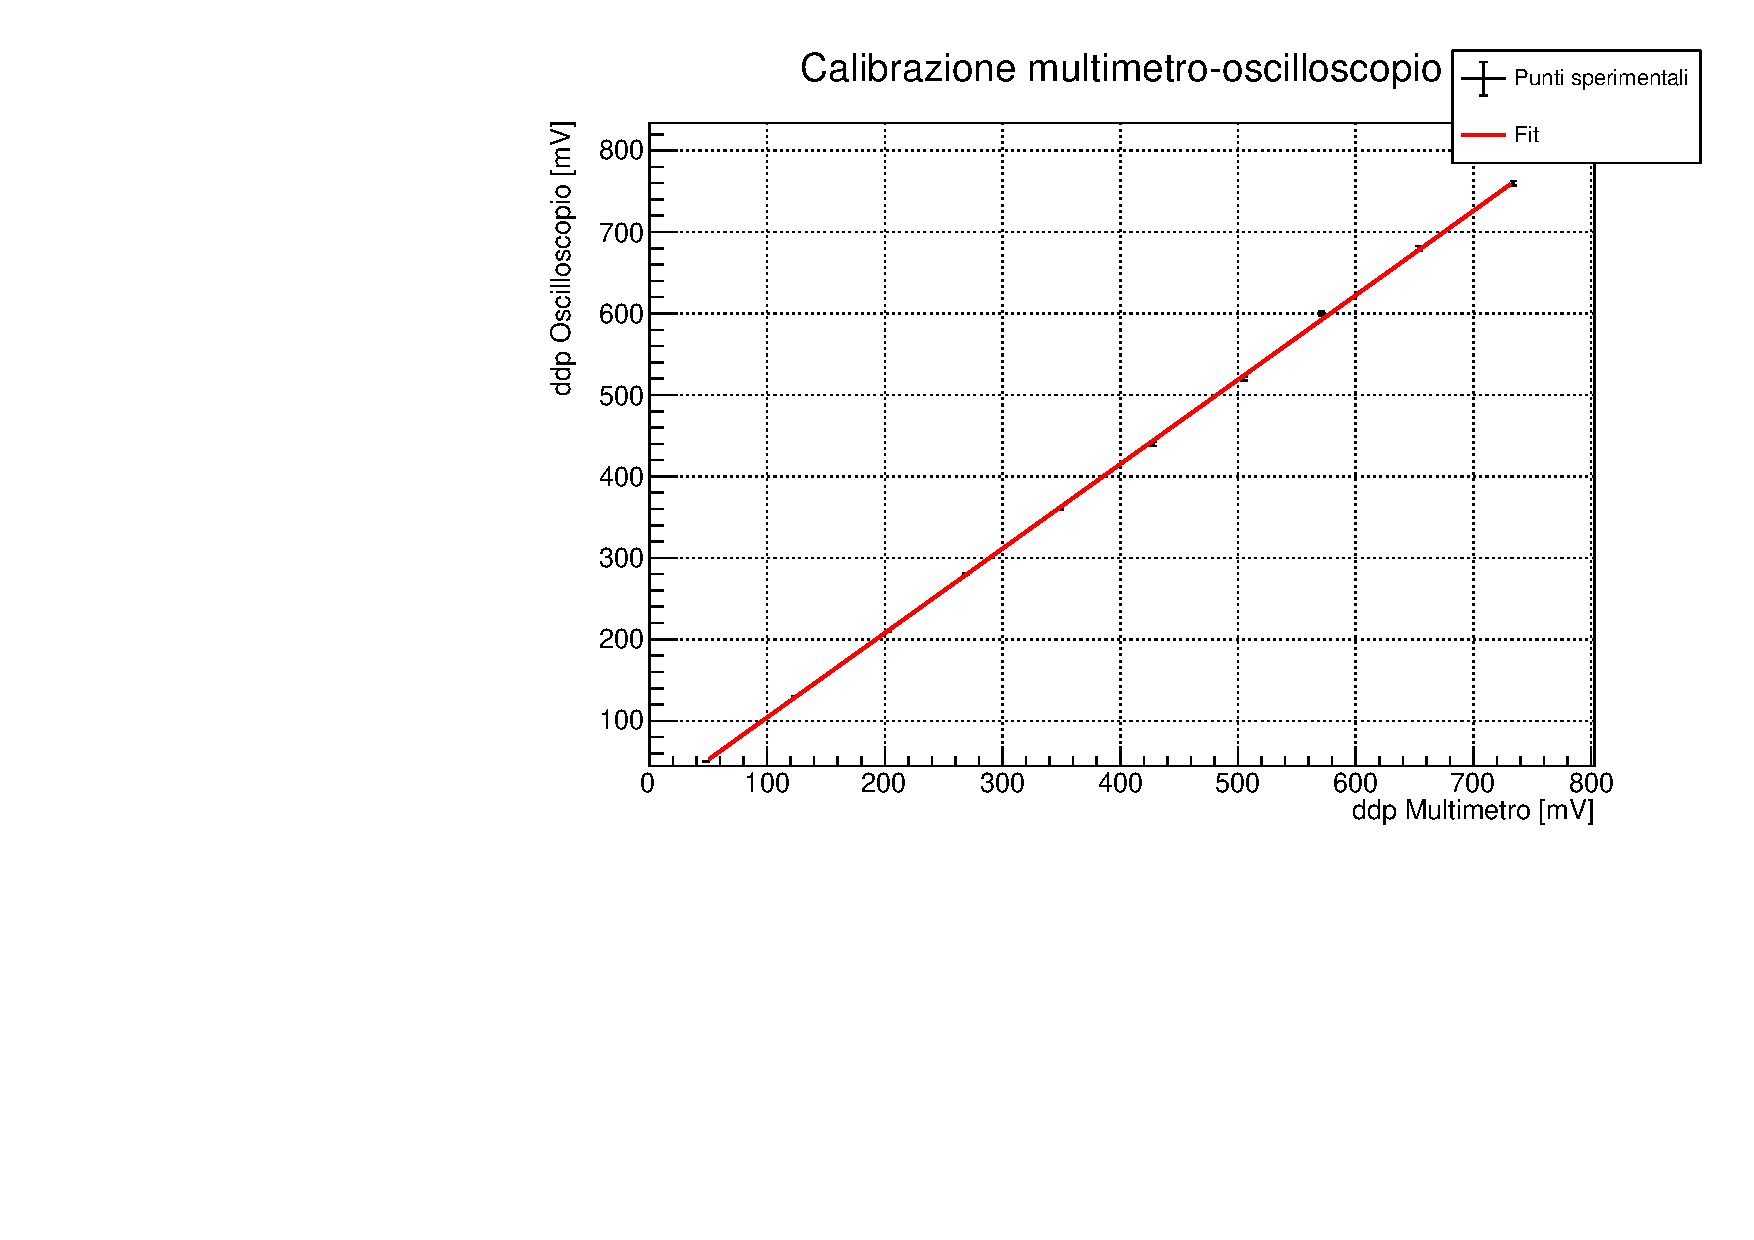
\includegraphics[width=0.6\linewidth]{../Silicio/Calibrazione}
	\caption{Retta di calibrazione delle tensioni dell'oscilloscopio}
	\label{fig:calibrazione}
\end{figure}	content...
\end{comment}
Questa misura ci ha permesso di considerare trascurabili eventuali errori dovuti alla calibrazione dello strumento poichè questi risultano chiaramente inferiori agli errori strumentali da noi valutati e riportati nelle tabelle (\ref{tab:silicio}) e (\ref{tab:germanio}).
\subsection{Silicio}
Dai dati in tabella (\ref{tab:silicio}), come già spiegato, abbiamo effettuato due fit, riportati graficamente in figura (\ref{fig:silicio}): quello esponenziale ci ha concesso di stimare $I_0=(5\pm5)mA$ e $\eta V_T=(51\pm5)mV$, mentre quello lineare ha restituito valori di $I_0=(7.2\pm0.7)mA$ e $\eta V_T=(53\pm4)mV$. Per entrambi i fit non abbiamo utilizzato tutti i punti sperimentali raccolti, ma abbiamo valutato quale fosse il range di fit migliore alla luce del fatto che dopo un certo valore di soglia il comportamento caratteristico muta dalla legge ideale, come è possibile apprezzare negli ultimi punti rappresentati, seppur non utilizzati, del grafico semilogaritimico in figura(\ref{fig:silicio}). 
\begin{comment}
	\begin{figure}[H]
		\centering
		\includegraphics[width=0.9\linewidth]{../Silicio/canvas}
		\caption{Caratteristica I-V del diodo al Silicio: a sinistra sono riportati i punti nel range utilizzato per effettuare il fit esponenziale mentre a destra sono riportati tutti i punti sperimentali in scala semilogaritmica con fit lineare}
		\label{fig:silicio}
	\end{figure}content...
\end{comment}
Osserviamo che le misure ottenute dai due fit sono compatibili tra loro seppur il fit lineare si riveli più preciso riuscendo a stimare con un errore minore il parametro $I_0$.
I parametri misurati si rivelano in questo caso in accordo con quelli attesi.
\subsection{Germanio}
I fit effettuati e riportati graficamente in figura (\ref{fig:germanio}) hanno concesso di stimare $I_0=(4\pm1)\mu A$ e $\eta V_T=(43\pm5)mV$ (fit esponenziale) e $I_0=(2.6\pm0.3)\mu A$ e $\eta V_T=(40\pm3)mV$ (fit lineare). Anche in questo caso per entrambi i fit non abbiamo usato tutti i punti sperimentali raccolti. In questo caso la deviazione dal comportamento ideale è ancor più evidente che con il diodo al Silicio, come si può apprezzare negli ultimi punti rappresentati, seppur non utilizzati, del grafico semilogaritimico in figura(\ref{fig:germanio}).
\begin{comment}
	\begin{figure}[H]
		\centering
		\includegraphics[width=0.9\linewidth]{../Germanio/canvas}
		\caption{Caratteristica I-V del diodo al Germanio: a sinistra sono riportati i punti nel range utilizzato per effettuare il fit esponenziale mentre a destra sono riportati tutti i punti sperimentali in scala semilogaritmica con fit lineare}
		\label{fig:germanio}
	\end{figure}content...
\end{comment}
Anche in questo caso osserviamo che le misure ottenute dai due fit sono compatibili tra loro seppur il fit lineare si riveli più preciso riuscendo a stimare con un errore minore il parametro $I_0$.
Notiamo però che il parametro misurato $\eta V_T$ non risulta in accordo con quello atteso; questo è dovuto a vari fattori tra cui l'impossibilità di misurare la temperatura di operazione della giunzione che varia il valore di questo parametro.
\section*{Conclusioni}
Le misure della caratteristica I-V dei due diodi si sono rivelate qualitativamente in accordo con la teoria riproducendo la legge del diodo ideale e manifestando anche una minor aderenza con questa a tensioni più alte, come è previsto dalla caratteristica di un diodo reale. 

Per il diodo al Silicio abbiamo ottenuto due misure di ogni parametro caratteristico, $I_0=(5\pm5)mA$ e $\eta V_T=(51\pm5)mV$ con fit esponenziale, e $I_0=(7.2\pm0.7)mA$ e $\eta V_T=(53\pm4)mV$ con fit lineare, in accordo tra di loro ed entrambe in accordo con i valori attesi. Per quanto riguarda il diodo al Germanio il fit esponenziale ha restituito $I_0=(4\pm1)\mu A$ e $\eta V_T=(43\pm5)mV$, in accordo con le stime del fit lineare $I_0=(2.6\pm0.3)\mu A$ e $\eta V_T=(40\pm3)mV$, ma entrambi in disaccordo con i valori attesi. Questa discrepanza è dovuta alle variazioni di temperatura della giunzione che fanno variare il valore di $\eta V_T$, combinate con gli errori strumentali.
\end{document}
